%=================================================================
\documentclass{amsart} 


\newtheorem{theorem}{Theorem}[section]
\newtheorem{proposition}[theorem]{Proposition}
\newtheorem{lemma}[theorem]{Lemma}
\newtheorem{corollary}[theorem]{Corollary}
\newtheorem{assumption}[theorem]{Assumption}
\newtheorem{remark}[theorem]{Remark}

\newcounter{example}
\theoremstyle{definition}
\newtheorem{example}[theorem]{Example}

\numberwithin{equation}{section}

\usepackage{paralist}
\usepackage[hidelinks]{hyperref}


\usepackage{booktabs}
\usepackage{cite}
\usepackage{enumitem}
\usepackage{float}
\usepackage{amssymb}
\usepackage{mathtools}
\usepackage{url}
% for algorithms
\usepackage[linesnumbered,ruled,vlined]{algorithm2e}
\usepackage{csquotes}
\newcommand{\Vvert}{{\vert\kern-0.25ex\vert\kern-0.25ex\vert}}
\usepackage{tikz,pgfplots}
\pgfplotsset{select coords between index/.style 2 args={
		x filter/.code={
			\ifnum\coordindex<#1\def\pgfmathresult{}\fi
			\ifnum\coordindex>#2\def\pgfmathresult{}\fi
		}
}}

%========================
\usepackage{textcomp}
\hbadness=10000
\vbadness=10000
\usepackage[textsize=tiny]{todonotes}
\newcommand{\cA}{\mathcal{A}}
\newcommand{\cB}{\mathcal{B}}
\newcommand{\cL}{\mathcal{L}}
\newcommand{\cP}{\mathcal{P}}
\newcommand{\cU}{\mathcal{U}}
\newcommand{\cV}{\mathcal{V}}
\newcommand{\cW}{\mathcal{W}}
\newcommand{\cX}{\mathcal{X}}
\newcommand{\cY}{\mathcal{Y}}
\newcommand{\cZ}{\mathcal{Z}}

\newcommand{\R}{\mathbb{R}}
\newcommand{\X}{\mathbb{X}}
\newcommand{\Y}{\mathbb{Y}}

% extension and restriction operator
\newcommand{\Ext}{E}
\newcommand{\Res}{R}
% adjoints
\newcommand{\aExt}{E'}
\newcommand{\aRes}{R'}

\newcommand{\EBox}{\Ext_{\Omega\rightarrow\square}}
\newcommand{\RBox}{\Res_{\Omega\leftarrow\square}}

\newcommand{\aEBox}{\aExt_{\Omega\leftarrow\square}}
\newcommand{\aRBox}{\aRes_{\Omega\rightarrow\square}}

\newcommand{\ECirc}{\Ext_{\mycirc\rightarrow\Omega}}
\newcommand{\RCirc}{\Res_{\mycirc\leftarrow\Omega}}

\newcommand{\aECirc}{\aExt_{\mycirc\leftarrow\Omega}}
\newcommand{\aRCirc}{\aRes_{\mycirc\rightarrow\Omega}}

%-----
% now space-time

\newcommand{\EstBox}{\Ext_{I\times\Omega\rightarrow I\times\square}}
\newcommand{\RstBox}{\Res_{I\times\Omega\leftarrow I\times\square}}

\newcommand{\astEBox}{\aExt_{I\times\Omega\leftarrow I\times\square}}
\newcommand{\astRBox}{\aRes_{I\times\Omega\rightarrow I\times\square}}

\newcommand{\EstCirc}{\Ext_{I\times\mycirc\rightarrow I\times\Omega}}
\newcommand{\RstCirc}{\Res_{I\times\mycirc\leftarrow I\times\Omega}}

\newcommand{\astECirc}{\aExt_{I\times\mycirc\leftarrow I\times\Omega}}
\newcommand{\astRCirc}{\aRes_{I\times\mycirc\rightarrow I\times\Omega}}


%\usepackage{relsize}
%\newcommand*{\mycirc}{\mathrel{\scalebox{0.8}{$\bigcirc$}}}
\usepackage{wasysym}
\newcommand{\mycirc}{\text{\Circle}}

% identity operators
\DeclareMathOperator{\id}{id}
\DeclareMathOperator{\dom}{dom}
\DeclareMathOperator{\range}{range}

% limiters
\DeclarePairedDelimiter{\dual}{\langle}{\rangle}
%========================
% reduce space below figures
\setlength{\belowcaptionskip}{-10pt}
%========================
\begin{document}

\title[A posteriori ertification for PINNs]{A posteriori Certification for physics-informed neural networks}

\author{Lewin Ernst}
\address{Institute for Numerical Mathematics, Ulm University, Helmholtzstr. 20, 89081 Ulm, Germany}
\email{lewin.ernst@uni-ulm.de}

\author{Nikolaos Rekatsinas}
\address{Institute of Applied and Computational Mathematics, Foundation of Research and Technology, Nikolaou Plastira 100, Vassilika Vouton,
GR 70013 Heraklion, Crete, Greece}
\email{n.rekatsinas@iacm.forth.gr}

\author{Karsten Urban}
\address{Institute for Numerical Mathematics, Ulm University, Helmholtzstr. 20, 89081 Ulm, Germany}
\email{karsten.urban@uni-ulm.de}


\begin{abstract}
	We propose rigorous lower and upper bounds for a PINN approximation to PDEs by efficiently computing the Riesz representations of suitable extension and restrictions of the PINN residual towards geometrically simpler domains, which are either embedded or enveloping the original domain. Error bounds are proven and detailed for elliptic as well as parabolic problems. Numerical experiments show the good quantitative behaviour of the derived upper and lower error bounds.
\end{abstract}

\keywords{
	Physics Informed Neural Networks; A Posteriori Error Bound; Parameterized Partial Differential Equations; Extension and Restriction of Functionals}

\subjclass{35J20, % Variational methods for second-order elliptic equations
	65M15, % Error bounds 
	68T07% Artifcial neural networks and deep learning
}


\maketitle

\documentclass[../main.tex]{subfiles}
\graphicspath{{../images/}}
\makeatletter
\def\input@path{{../images/}}
\makeatother
\begin{document}
\section{Introduction}
\begin{figure}
\centering
\begin{tikzpicture}
\node[inner sep=0pt] (ws) at (0, 0) {
\includegraphics[height=.4\textwidth, trim={10cm 0 10cm 0},clip]{world_space.png}};
\node[inner sep=0pt] (cs) at (6,0) {\includegraphics[height=.4\textwidth, trim={10cm 1cm 10cm 4cm},clip]{conf_space.png}};
\end{tikzpicture}
\vspace{-5pt}
\label{fig:pbrm_intro}
\caption{\textbf{Left}: Shows world space obstacles as grey spheres. Robots start and goal configuration is colored red and green, respectively. Configurations along the computed path are colored transparent blue. \textbf{Right:} Mapped world space scenario to configuration space. Obstacle region is the grey mesh. Red spheres are collision-free regions computed by the neural SCDF. The optimized shortest path in the convex corridor is the blue curve.}
\vspace{-25pt}
\end{figure}
Motion planning is the problem of finding a collision-free trajectory that connects a given start and goal configuration. The planning takes place in the configuration space of the robot. For single body robots, like mobile robots or drones, the configuration space and the world space are usually the same. This simplifies the planning, since explicit obstacle representations are available which enables geometrical tools like separating hyperplanes, smallest distance to obstacles etc., to be used when designing motion planning algorithms. For multi-body robots like manipulators, the situation is completely different. The world space obstacles are usually mapped to non-convex regions, and to make the problem even harder, the mapping is usually not known. Forming explicit representations of the obstacle region in the configuration space is usually too expensive or intractable. Despite all of this, sampling based planners are used with great success, which mainly is due to their use of implicit representations of the obstacle region. The basic idea is to construct a graph in the configuration space that covers and connects the collision-free region. From this graph, a path can be extracted that connects a given start and goal configuration. The approach is computationally expensive, since the graph is constructed with the smallest geometrical building block available, points, which represents a collision-check. Furthermore, the extracted paths from the graph are non-smooth and jagged due to the stochastic nature of the approach. This adds an additional post-processing step to the process, where the paths are shortcutted and smoothened, before the path can be used for tracking. Clearly a lot of time is invested to form this graph and produce smooth paths. Thus, if the obstacles start to move, then all of this work is done in no use, since all points that make up this graph need to be re-verified, which is simply too time consuming to be done in real time.
\\\\
In this work, we want to address the existing drawbacks of the sampling based planners. Our main contribution is an improved motion planner where each vertex in the graph covers a collision-free region in the form of a sphere instead of a point and where the edges are formed with neighboring intersecting spheres. This representation has the advantage of instead of returning piecewise linear paths, returning a sequence of overlapping spheres, i.e. a convex corridor, that connects a given start and goal configuration, illustrated in Figure \ref{fig:pbrm_intro}. This convex corridor allows us to use convex optimization to produce smooth trajectories, instead of computationally expensive post-processing methods. The representation further allows us to estimate the coverage of the collision-free space, which gives us awareness and feedback in the offline roadmap construction phase. Finally, our representation is simple to adapt to moving obstacles, simply requery for the new radii and recheck for intersections. 
\\\\
The spherical collision-free regions are formed using a signed distance function (SDF), which is a function that returns the smallest distance from an arbitrary point to the boundary of an obstacle. As the name implies, the distance is signed, thus if the point is inside the obstacle it is negative otherwise positive. If the distance is positive, a sphere with radius equal to the distance is guaranteed to cover a collision-free region. Using an SDF in motion planning is not new, but what is novel about our approach is that we express the distance in the configuration space instead of the world space and by doing so allows us to form these convex collision-free regions. We refer to the resulting SDF as a signed configuration distance function (SCDF). Computing an SCDF analytically is non-trivial, our approach is therefore to parameterize the SCDF with a deep neural network and learn the mapping by supervised learning. Our resulting neural SCDF can compute distances for different parameter values of obstacle shapes and we also show how multiple distances can be combined, thus making our approach flexible.
\section{Related work}
Motion planning algorithms can roughly be divided into three families, grid-based, sampling based and optimization based methods. Grid-based methods (GBM) discretize the planning space from which a graph is then compiled. A standard search method is A$^\star$ \citep{a_star}, which is classified as an \textit{informed} search method, since it employs a heuristic function to speed up the search. A$^\star$ guarantees to return an optimal path at the level of discretization used. GBMs usually discretize the planning space by a regular lattice and this limits the GBMs to problems with low dimensionality due to the curse of dimensionality. Thus, GBMs are usually limited to single-body robots where the degrees of freedom (DOF) are low. To overcome the inherent scaling problem with the GBMs, stochastic methods are usually used for multi-body robots. These methods are termed as sampling-based methods (SBM) and core members within this family are the rapidly-exploring random trees (RRT) \citep{rrt} and the probabilistic roadmap (PRM) \citep{prm}. RRT grows a tree from the start configuration and explores the collision-free region in a rapid way until it is able to connect to the goal region. RRT is usually improved by bi-directional planning \citep{rrt_connect}, i.e. an additional tree is grown from the goal configuration and the trees are tested for connection after any tree has been expanded. RRT is a single-query method, thus it searches for a path from scratch each time it is queried. Contrary to this, PRM is a multi-query method, which solves for multiple queries without starting from scratch. PRM does this by creating a roadmap (graph) that covers the collision-free space as an offline step. The graph is then used to solve for multiple queries. PRMs are used in cases where the environment does not change since the extra offline step is too computationally costly and needs to be re-done if the environment is changed. In our work, we address this inherent issue by using a different roadmap representation. Our vertices in the graph cover a collision-free region in the form of spheres and we form the edges by checking for intersecting spheres. If something in the environment changes, we recompute the spheres radii and recheck the intersections, without relying on collision detection. We use a trained neural network to compute the sphere radius, therefore querying for the radius can be done fast, hence our representation enables the PRM for dynamic environments.
\\\\
In the recent decades, optimization based methods (OBM) \citep{chomp, schulman, itomp, stomp} have been introduced as an alternative to SBM for multi-body robots. Like the SBM, the OBMs scale well to higher dimensional problems and produce smoother motion. It is common to use a SDF in the optimization since it is a smooth function, thus enabling gradient-based methods. However, the standard way of expressing the SDF is in world space. The distance therefore needs to be mapped to the configuration space by the forward kinematics. This mapping makes the optimization problem a non-linear program (NLP), which is computationally expensive to solve. Recently, a different approach has been proposed. In \cite{mp_gcs} motion planning is formulated as a convex optimization problem by using the graph of convex sets framework \citep{gcs}. The underlying idea is to decompose the collision-free space into intersecting convex sets from which a convex optimization problem is formulated. In cases where an explicit representation of the obstacles in the configuration space exists, like for single-body robots, creating collision-free convex regions can be done fast \citep{iris}. For multi-body robots, this is non-trivial. Existing work does this successfully \citep{iris_nlp, iris_c} by an optimization based approach, but the methods are still too time consuming to be used in the presence of moving obstacles. Our approach is instead to use deep learning to learn an SDF expressed in the configuration space. With this, we can query for shortest distances to the collision boundary, which allows us to expand spherical regions which are collision-free. Our approach is fast and therefore enables our suggested roadmap planner to be used in dynamic environments.
\\\\
Recent research has focused on learning collision detection \citep{fk_kernel_distance, diffco, graphdistnet} by predicting the signed distance between the robot links and the surrounding obstacles in the world space. The learned SDF is used in trajectory optimization but since the distance is expressed in the world space, the problem becomes an NLP and therefore takes a long time to solve. We take a novel approach and suggest to instead express the signed distance in the configuration space. This allows us to improve the PRM at the same time as it enables convex optimization for trajectory optimization, which runs faster and is more reliable than NLP solvers. In \cite{cspf} a learned signed distance function in the configuration space is proposed similar to our approach. However, their approach is restricted to point cloud representations, while we propose to represent the obstacles as parameterized geometric shapes, e.g. spheres. Furthermore, we also show how to use our learned SCDF to improve an existing roadmap planner.
\section{Problem formulation}
A robot is located in the world space, $\W \subset \R^3 $. The unique location of the robot is given by its configuration $\q \in \C$, where $\C$ is the configuration space. The set of points covered by the robots bodies at a certain configuration is expressed as $\B(\q) \subset \W$. The robot is surrounded by $\NrObst$ obstacles $\O = \bigcup_{i=1}^{\NrObst} \O_i$, where  $\O_i \subset \W$. The representation of the obstacle in the configuration space is the set $\C\O_i = \{\q \in \C \: |\: \B(\q) \cap \O_i \neq \emptyset \}$. The obstacle space is formed as $\Co = \bigcup_{i=1}^{\NrObst} \C \O_i$. The complement is referred to as the free space, $\Cf = \C \setminus \Co$. The path planning problem is a tuple, ($\Cf$, $\qStart$, $\qGoal$), where we want to connect a query pair, consisting of a start, $\qStart$, and goal configuration, $\qGoal$, with a geometric path, $\q(s): [0, 1] \mapsto \Cf$, such that $\q(0)=\qStart$ and $\q(1)=\qGoal$, or report correctly when such a path does not exist.
\end{document}

% !TEX root = ../dual_norm_estimate_base.tex

\section{PINNs for solving PDEs} \label{sec:PINNs}
We are going to briefly introduce the main concepts of PINNs without going into details, since we only aim to use PINNs as a black box.

\subsection{PDEs in classical form}
Let $\Omega \subset \mathbb{R}^d$ be a bounded open domain and let $m\in\mathbb{N}$ denote the order of the PDE ($m=2$ for Laplace's equation). We denote by
\begin{align*}
    B^\circ: C^m(\Omega)\to C^0(\Omega)
\end{align*}
the classical (point-wise) form of the differential operator under consideration. Then, given some $f^\circ\in C(\Omega)$, we call $u\in C^m(\Omega)$ a \emph{classical solution} if 
\begin{equation} \label{eq:clPDE}
	(B^\circ u)(x) = f^\circ(x), \quad \forall x \in \Omega,
\end{equation}
where we assume that proper boundary and/or initial conditions are incorporated into the definition of the operator.

Next, we are given some approximation $u^\delta$ to $u$, e.g.\ in terms of a PINN and define the (classical) \emph{residual} of \eqref{eq:clPDE} by
\begin{align}\label{eq:residual}
    r_\Omega^\circ (u^\delta)(x) := f(x) - (B^\circ u^\delta)(x), \quad x\in \Omega. 
\end{align}
Given $u^\delta$, the residual is in principle computable by inserting $u^\delta$ into the PDE operator.

However, such classical solutions often do not exist, depending on the data $B^\circ$, $f^\circ$ and $\Omega$. It is well-known that well-posedness of such problems is usually linked to suitable variational formulations as described in Section \ref{sec:VarFormPDEs} below. 


\subsection{PINNs: Definition and training}
The core idea of PINNs is to use the residual for the definition of a loss function within the training of a neural network. Let us briefly describe this for the above classical solution concept, even though (i) there are several other approaches in the literature and (ii) our subsequent error analysis does not depend on the choice of the loss function for a PINN.

\subsubsection*{Neural networks (NNs)} 
The notation of NNs in this paragraph is based upon \cite{Berner2021,Gribonval2021,Petersen2018}. A NN is a function $\Phi_a(\cdot;\theta):\mathbb{R}^{N_{0}} \rightarrow \mathbb{R}^{N_{L}}$, where $a$ is the \emph{architecture} and $\theta$ are the \emph{parameters}. Both the architecture and parameters determine the input-output function $\Phi_a(\cdot;\theta)$ of the NN. In case of a feed-forward NN, the architecture $a=(N,\rho)$ can be described by the vector of neurons per layer $N=(N_0,...,N_L)\in\mathbb{N}^{L+1}$, where $L \in \mathbb{N}$ denotes the number of \emph{layers} ($N_0$ being the input and $N_L$ the output dimension) and the \emph{activation function} $\rho: \mathbb{R} \rightarrow \mathbb{R}$.

The parameters of the NN read $\theta = (W^{(l)},b^{(l)})_{l=1,...,L}$, where $W^{(l)} \in \mathbb{R}^{N_{l} \times N_{l-1}}$ are the \emph{weight matrices} and $b^{(l)} \in \mathbb{R}^{N_{l}}$ are called \emph{bias vectors}. 
The output $\Phi_a(z;\theta)$ of the NN for an input $z\in\mathbb{R}^{N_0}$ is then defined as $\Phi_{a}(z;\theta) := \Phi^{(L)}(z;\theta)$, where
\begin{align*}
	\Phi^{(1)}(z;\theta) &= W^{(1)} z + b^{(1)}, \\
	\hat{\Phi}^{(l)}(z;\theta) &= \rho(\Phi^{(l)}(z;\theta)), \quad l=1,...,L-1, \quad \text{and} \\
	\Phi^{(l+1)}(z;\theta) &= W^{(l+1)} \hat{\Phi}^{(l)}(z;\theta) + b^{(l+1)}, \quad l = 1,...,L-1,
\end{align*}
and $\rho$ is applied component-wise. In the following the architecture is omitted in the notation as we view it as being fixed once and for all. 

NNs seem suitable for solving PDEs because they are universal function approximators, see \cite{Hornik1991,Hornik1989,Guehring2019}. For a NN $\Phi^\theta := \Phi(\cdot;\theta)$ to approximate the solution of a PDE, the parameters $\theta$ must be determined, which is done in the training phase. Thereby, a tailored minimization problem is defined, with which the parameters are \emph{learned}. In the regime of PINNs the function to be minimized involves the PDE (e.g.\ in classical form \eqref{eq:clPDE}), which is the reason for the name \emph{physics-informed}.

With respect to the classical form of the PDE, a set of sample points $\mathcal{S}_\Omega$ in $\Omega$ are chosen and \eqref{eq:clPDE} is posed only for those points. This leads to the definition of the loss function
\begin{equation}\label{eq:lossfunc}
	\mathcal{L}(\theta) 
    := \sum_{x \in \mathcal{S}_\Omega} 
    \vert (r^\circ_\Omega (\Phi^\theta))(x) \vert^2.
\end{equation}
Often, an additional sampling is required for satisfying the boundary conditions. We shall assume that $\Phi^\theta$ satisfies given boundary condition as this can be achieved with the aid of approximate distance functions, see \cite{sukumar2022exact}. 

Such classical PINNs have e.g.\ been investigated for a broad scope of linear and nonlinear PDEs, see e.g. \cite{Berg2018,Raissi2019,Mao2020,Cai2021,Cai2021a,Hu2024}. The main advantages of the method are its straightforward applicability and, due to the sampling of $\mathcal{S}_\Omega$, it results in a mesh-free approximation. 

One can also replace the above loss function by terms stemming from a variational formulation of a given PDE, e.g.\ VPINNs. Again, as the specific form of the PINN is not relevant for our paper, we will not go into more details and only assume that $\Phi^\theta$ gives some approximation for the solution of a given PDE.

% !TEX root = ../dual_norm_estimate_base.tex

\section{Error-residual relations for PDEs} \label{sec:VarFormPDEs}
In this section, we recall the main facts on error-residual relations for PDEs, which is based upon the well-known Hilbert space theory of PDEs yielding well-posed formulations.

\subsection{Well-posedness}
Given a partial differential operator $B$ (eventually starting from a classical version $B^\circ$), we require Hilbert spaces $\cW$, $\cY$ with norms $\|\cdot\|_\cX$ induced by inner products $(\cdot,\cdot)_\cX$, $\cX\in\{\cW,\cY\}$, such that  the PDE
\begin{equation} \label{eq:generalPDE}
	B u  = f
\end{equation}
is \emph{well-posed} for any appropriate right-hand side $f$, by which we mean that \eqref{eq:generalPDE} admits a unique solution, which continuously depends on the data (typically the right-hand side $f$). In order to ensure this, the domain $\cW$ and the range $\cY'$ of the operator $B$ have to be identified such that $B \in \cL_{\text{is}}(\cW, \cY')$\footnote{The space $\cL_{\text{is}}(\cW, \cY')$ is the subspace of isomorphisms from $\cL(\cW, \cY')$, where $(\cL(\cW, \cY'), \Vert \cdot \Vert_{L(\cW, \cY')})$ denotes the space of continuous linear functions from $\cW$ to $\cY'$.}, where $\cY'$ is the topological dual space of $\cY$ equipped with the operator norm 
\begin{equation*}
	\Vert f \Vert_{\cY'} 
    := \sup_{v \in \cY} \frac{f(v)}{\Vert v \Vert_{\cY}}
    = \sup_{v \in \cY} \frac{\langle f, v\rangle_\cY}{\Vert v \Vert_{\cY}},
    \end{equation*} 
i.e.,  $\langle \cdot,\cdot\rangle_\cY\equiv \langle \cdot,\cdot\rangle_{\cY'\times\cY}$ denotes the dual pairing. The reason why we choose the dual $\cY'$ for the range of $B$ lies in the fact that this easily allows one to relate the differential operator to a bilinear form
\begin{align*}
    b:\cW\times\cY\to\mathbb{R}
    \quad\text{via}\quad
    b(w,y) := \langle Bw,y\rangle_{\cY},
    \,\, w\in\cW, y\in\cY.
\end{align*}
 If $B\in\cL_{\text{is}}(\cW, \cY')$, the operator is bijective, which ensures existence and uniqueness for all $f\in\cY'$. Moreover, the inverse is bounded, i.e., 
\begin{align*}
    \Vert B^{-1} \Vert_{\cL(\cY', \cW)} < \infty,
\end{align*}
which will be relevant next.

Assume that we are given some approximation $u^\delta$ of the (exact, but typically unknown) solution $u\in\cW$, e.g.\ determined by some PINN. Then, we are interested in controlling the error $\Vert u - u^{\delta} \Vert_{\cW}$. If $B \in \cL_{\text{is}}(\cW, \cY')$, one can bound  the error by the dual norm of the \emph{residual} $r_B(u^\delta) := f - Bu^\delta\in\cY'$ as
\begin{equation} \label{eq:ErrorResiLinearV1}
	\Vert B \Vert^{-1}_{\cL(\cW, \cY')} \cdot \Vert r_B(u^{\delta}) \Vert_{\cY'} 
    \,\le\, 
    \Vert u - u^{\delta} \Vert_{\cW} 
    \,\le\, 
    \Vert B^{-1} \Vert_{\cL(\cY', \cW)} \cdot \Vert r_B(u^{\delta}) \Vert_{\cY'}
\end{equation}
The constants $c_B:=\Vert B \Vert_{\cL(\cW, \cY')}^{-1} >0 $ on the left and $C_B:=\Vert B^{-1} \Vert_{\cL(\cY', \cW)} <\infty$ on the right of \eqref{eq:ErrorResiLinearV1} are the (inverse of the) continuity and stability (inf-sup) constants, respectively. Then, \eqref{eq:ErrorResiLinearV1} reads
\begin{equation} \label{eq:ErrorResiLinearV2}
	c_B \, \Vert r_B(u^{\delta}) \Vert_{\cY'} 
    \,\le\, 
    \Vert u - u^{\delta} \Vert_{\cW} 
    \,\le\, 
    C_B \, \Vert r_B(u^{\delta}) \Vert_{\cY'}, \quad \forall u^\delta \in \cW.
\end{equation}
Hence, we can bound the error from above and from below by the residual, if we
\begin{compactitem}
    \item  either know or are able to compute or estimate the continuity and stability constants and
    \item are able to evaluate the dual norm of the residual, i.e.
    \begin{equation*}
	\Vert r_B(u^{\delta}) \Vert_{\cY'} = \sup\limits_{v \in \cY} \frac{\langle r_B(u^{\delta}), v \rangle_{\cY}}{\Vert v \Vert_\cY}.
    \end{equation*}
    However, the computation of the supremum is in general not possible.
\end{compactitem}

\subsection{PDEs on domains}
The above introduced abstract spaces $\cW$ and $\cY$ are typically function spaces which are defined upon a physical domain $\Omega \subset \mathbb{R}^d$, on which the PDE is posed. Hence, we sometimes use the notations $\cW(\Omega)$ and $\cY(\Omega)$, also for domains different from the original $\Omega$. Boundary and/or initial conditions are incorporated into the definition of the operator $B$. It will be important later to keep track on the domain $\Omega$.


\begin{example}[Linear elliptic PDE]\label{example:linearPDE}
	Let $\Omega \subset \mathbb{R}^d$ be a Lipschitz domain and let $\cW=\cY=H^1_0(\Omega)$. Given $f\in H^{-1}(\Omega)$, the problem of finding $u \in H^1_0(\Omega)$ satisfying 
	\begin{equation*}
		\langle Bu,v\rangle_{H^1_0(\Omega)} := (A \nabla u, \nabla v )_{L_2(\Omega)} + (b \cdot \nabla u, v)_{L_2(\Omega)} + (c \cdot u, v)_{L_2(\Omega)} = f(v)
	\end{equation*}
	for all $ v \in H^1_0(\Omega)$ is well-posed, if $A \in \left(L_\infty(\Omega)\right)^{d \times d}$, $b \in \left(L_\infty(\Omega)\right)^{d}$, $c \in L_\infty(\Omega)$ and
	\begin{equation*}
		\nabla \cdot b \in L_2(\Omega), \quad c(x) 
        - \tfrac{1}{2} \nabla \cdot b(x) \ge c_0 \quad \forall x \in \Omega \; \text{ a.e. }
	\end{equation*}
	as well as 
	\begin{equation*}
		\xi^T A(x) \xi \ge a_0 \vert \xi \vert^2, \quad \forall \xi \in \mathbb{R}^{d} \; \forall x \in \Omega \; \text{ a.e.,}
	\end{equation*}	
    i.e., $A$ is s.p.d. 
    In this case \eqref{eq:ErrorResiLinearV2} holds with $c = (\Vert A \Vert_\infty + s_{\text{PF}} \Vert b \Vert_\infty + s_{\text{PF}}^2 \Vert c \Vert_\infty)^{-1}$ and $C = a_0^{-1}$, whereby $s_{\text{PF}}$ is the Poincar\'{e} constant for $\Omega$.\hfill$\diamond$
\end{example}

\begin{example}[Space-time variational form of parabolic PDEs]\label{Ex:SpaceTime}
    Let the PDE operator $A\in\cL_{\text{is}}(W(\Omega),Y'(\Omega))$ be well-posed on some domain $\Omega\subset\mathbb{R}^d$ for appropriate function spaces $W(\Omega)$ and $Y(\Omega)$. Then, given $f\in\cY'=L_2(I;Y'(\Omega)):=\{ g:I\to Y'(\Omega): \| g\|_{L_2(I;Y'(\Omega))}^2:=\int_T \| g(t)\|_{Y'(\Omega)}^2\, dt<\infty\}$, we seek a solution $u\in\cW$ (with $\cW$ to be defined) of the evolution problem $Bu:=\dot{u}+Au=f$ in $\cY'$ and $u(0)=0$. It is well-known that the Bochner space $\cW:=\{ w\in L_2(I;W(\Omega)): \dot{w}\in L_2(I;W'(\Omega)), w(0)=0\}$ equipped with the graph norm $\Vert u \Vert_{\cW}^2 := \Vert \partial_t u \Vert_{L_2(I,W'(\Omega))}^2 + \Vert u \Vert_{L_2(I,W(\Omega))}^2$
    yields $B\in\cL_{\text{is}}(\cW,\cY')$, \cite{lions2000mathematical,schwab2009space}. This is known as the space-time variational formulation of parabolic PDEs, see also \cite{CheginiStevenson,SpaceTimeUrbanPatera}. If $A$ is elliptic, one has $W(\Omega)=Y(\Omega)=H^1_0(\Omega)$.
    \hfill$\diamond$
\end{example}

\subsection{Dual norm estimates}
We will now address the problem of finding a computable surrogate for the dual norm of the residual for well-posed PDE operator equations. To simplify the notation we consider general functionals $f \in \cY'$ instead of the residual $r_\Omega(u^\delta)$. We want to calculate or estimate the dual norm of the functional $f \in \cY'$, i.e., we seek a feasible surrogate $\eta(f)$ such that either
\begin{subequations}\label{eq:dualnorm}
\begin{align}
	\eta(f)  
        &=\Vert f \Vert_{\cY'}, 
        && \text{(identity)}
        \label{eq:dualnormEqual}\\
	\exists\, C,c >0:\quad c \, \eta(f)
        &\le \Vert f \Vert_{\cY'} 
        \le C \, \eta(f), \quad \text{or} 
        && \text{(estimate)}
        \label{eq:dualnormEst} \\
	\exists\, C > 0:\quad  \Vert f \Vert_{\cY'} 
        &\le C \, \eta(f) 
        && \text{(bound)}
        \label{eq:dualnormUpEst}
\end{align}
\end{subequations}
holds. Ideally, we find $\eta(f)$ such that identity \eqref{eq:dualnormEqual} is fulfilled, but this is typically not possible. Hence, one resorts to an estimate \eqref{eq:dualnormEst}, which ensures that $\eta(f)$ encloses the desired quantity and $\Vert f \Vert_{\cY'}$ is small if and only if $\eta(f)$ is. If this is still not achievable, a bound \eqref{eq:dualnormUpEst}, if not too loose, guarantees at least that the desired quantity is below a threshold, if the bound is so. 

By applying \eqref{eq:dualnormEqual} or \eqref{eq:dualnormEst} to \eqref{eq:ErrorResiLinearV2}, the error is controlled by $\eta$ as
\begin{equation*}
	c \cdot \eta \left( r_\Omega(u^\delta) \right) \le \Vert u - u_{\delta} \Vert_{\cW} \le C \cdot \eta \left( r_\Omega(u^\delta) \right), \quad c, C > 0
\end{equation*}
or by using \eqref{eq:dualnormUpEst} we have
\begin{equation*}
	\Vert u - u_{\delta} \Vert_{\cW} \le C \cdot \eta \left( r_\Omega(u^\delta) \right), \quad C > 0.
\end{equation*}
Notice that the constants $c$ and $C$ in the last two equations could be different to those of \eqref{eq:ErrorResiLinearV2}.

In the next section we shall describe how to find an efficient surrogate $\eta$ for PINNs, such that one of the equations \eqref{eq:dualnorm} is satisfied. It is clear that the structure of the underlying space $\cY$ is crucial for the derivation. 

\subsection{Riesz representation} \label{subsec:RieszReps}
Since $\cY$ is a Hilbert space, the Riesz Representation Theorem\,(see e.g. \cite{aubin2011applied}) states that $\eta(f)$ fulfilling \eqref{eq:dualnormEqual} is given by
\begin{equation*}
	\eta(f) := \Vert R^{-1}_{\cY} f \Vert_{\cY},
\end{equation*}
where $R_\cY: \cY \rightarrow \cY'$ denotes the Riesz-operator defined through the equation $(u, v)_\cY = \langle R_{\cY} u, v \rangle_{\cY}, \; u, v \in \cY$, where $(\cdot,\cdot)_\cY$ denotes the inner product in $\cY$. The Riesz representative $\hat{f} := R^{-1}_{\cY} f \in \cY$ is found by solving the equation
\begin{equation} \label{eq:RieszRep}
	(\hat{f}, v)_\cY = f(v), \quad \forall v \in \cY.
\end{equation}
Since $R_\cY$ is isometric we have $\eta(f) = \Vert f \Vert_{\cY'}$ and thus \eqref{eq:dualnormEqual}. Usually, evaluating $\Vert \cdot \Vert_{\cY}$ is much easier than evaluating $\Vert \cdot \Vert_{\cY'}$. Unfortunately, calculating the Riesz representative with \eqref{eq:RieszRep} is still unfeasible because the space $\cY$ is in almost all cases infinite-dimensional. Therefore, $\cY$ is replaced by a sufficiently high but finite-dimensional subspace $\cY^\delta \subset \cY$, e.g., a finite element space. The Riesz representative $\hat{f} \in \cY$ is then approximated by $\hat{f}^\delta \in \cY^\delta$, which is the solution of
\begin{equation} \label{eq:RieszRepFinite}
	(\hat{f}^\delta, v^\delta)_\cY = f(v^\delta), \quad \forall v^\delta \in \cY^\delta.
\end{equation}

\begin{remark}
If $\cY$ is not a Hilbert, but only a Banach space, the Riesz Representation Theorem is not applicable. However, one way out is to use wavelet methods to directly bound the dual norm $\Vert f \Vert_{\cY'}$ as proposed in\,\cite{ernst2024certified}. 
\end{remark}

With an increasing dimension of $\cY^\delta$ we can at least hope to have convergence of $\hat{f}^\delta $ to $\hat{f}$ in $\cY$ and therefore convergence of $\Vert \hat{f}^\delta \Vert_{\cY}$ to $\Vert f \Vert_{\cY'}$. The drawback of this approach is that, in the case of finite elements, the space $\cY^\delta$ requires a discretization of the underlying domain $\Omega$.


\section{Theoretical Results}
\label{sec:appendixTheoretical}

For this section, we use an alternate notation, replacing $\beta$ with $\eta= \frac{\beta}{1-\beta_o}$ to make the equations easier to read, such that:
\begin{align*}
    (1-\beta)U + \beta F \Leftrightarrow U + \eta F
\end{align*}

This does not affect the allocation made by the ILP, as it only scales all Q-values by $1/(1-\beta)$. This would only be undefined when $\beta=1$, but we avoid that condition in our proofs. As $\beta\rightarrow1, \eta\rightarrow\infty$, and for any $\beta'>\beta$, $\eta'>\eta$. Note that in the theorem statements, we replace $\beta$ with $\eta$, but the proofs are equivalent.

The following results hold for any fairness function used in the DECAF formulation.

\begin{proposition}
As $\eta_{test}\xrightarrow{} 0$, all fair-only models behave in a utility-maximizing manner.
\end{proposition}
We state this without proof. It is easy to follow how this holds, as at $\eta=0$, the fairness model does not play any role in the decision making.

\setcounter{theorem}{0}
\begin{theorem}
Given perfect estimates for utility and fairness, increasing $\eta$ always improves the one-step fairness gain for SO with $\gamma=0$.
\label{th:theorem_fair_app}
\end{theorem}
\begin{proof}
We assume that the utility and fairness estimators are converged, i.e., the estimates of fairness and utility are correct. For the following discussion, assume the environment has evolved over some time $t$ and is at a state $s_t$. We consider what changes when we change $\eta$ at this state. Variables used henceforth are conditioned on $s_t$, wherever reasonable. We make the conditioning on $s_t$ implicit and do not notate it, to make it easier to read.

With $\gamma=0$, the optimal utility and fairness estimates equal the one-step return, i.e. the change in utility and fairness because of the resulting joint action. Note that these values are not known to the agents prior to the allocation as they depend on the joint actions of all agents, so computing these estimates is not trivial.

Let $U_{tot}(\mathcal{A})$ and $F_{tot}(\mathcal{A})$ be defined as follows, given an allocation $\mathcal{A}$:
\begin{align}
    U_{tot}(\mathcal{A}) &= \sum_{i\in\alpha}U(\mathcal{A}_i)\\
    F_{tot}(\mathcal{A}) &= \sum_{i\in\alpha}F(\mathcal{A}_i)
\end{align}
We remind the reader that $\mathcal{A}_i$ refers to the action assigned to agent $i$ in the allocation $\mathcal{A}$.

Let $\textbf{Z}_t$ represent the agent metrics at time $t$. Further, let $\mathcal{A}^*$ represent the optimal allocation from the ILP with $\eta$ as the trade-off weight. Since $\mathcal{A}^*$ is optimal, it follows that for all other possible allocations $\mathcal{A}_o$: 
\begin{align}
    U_{tot}(\mathcal{A}^*) + \eta F_{tot}(\mathcal{A}^*) &\ge U_{tot}(\mathcal{A}_o) + \eta F_{tot}(\mathcal{A}_o)  \\
    U_{tot}(\mathcal{A}^*) - U_{tot}(\mathcal{A}_o)&\ge  \eta (F_{tot}(\mathcal{A}_o) - F_{tot}(\mathcal{A}^*)) \label{eq:base_comp} 
\end{align}

We are interested in finding what happens to the allocation when we increase $\eta$.
For $\eta'>\eta$, note that the left side of Eq.~\ref{eq:base_comp} remains the same. Since utility estimates are not affected by changing $\eta$, any other allocation $\mathcal{A}_o$ can only be selected over $\mathcal{A}^*$ if the following condition holds:
\begin{align}
    U_{tot}(\mathcal{A}^*) + \eta' F_{tot}(\mathcal{A}^*) &\le U_{tot}(\mathcal{A}_o) + \eta' F_{tot}(\mathcal{A}_o)  \\
    U_{tot}(\mathcal{A}^*) - U_{tot}(\mathcal{A}_o)&\le  \eta' (F_{tot}(\mathcal{A}_o) - F_{tot}(\mathcal{A}^*)) \label{eq:base_comp2} 
\end{align}

Combining Eqs.\ref{eq:base_comp} and \ref{eq:base_comp2}, we get the following:
\begin{align}
    \eta (F_{tot}(\mathcal{A}_o) - F_{tot}(\mathcal{A}^*)) &\le  \eta' (F_{tot}(\mathcal{A}_o) - F_{tot}(\mathcal{A}^*)) \\
    F_{tot}(\mathcal{A}^*)(\eta'-\eta) &\le F_{tot}(\mathcal{A}_o)(\eta'-\eta) \label{eq:base_comp3} 
\end{align}
Since $\eta\ge0$ and $\eta'>\eta$, Eq.~\ref{eq:base_comp3} can only be true if $F_{tot}(\mathcal{A}_o)>F_{tot}(\mathcal{A}_o)$.

Thus, any allocation $\mathcal{A}_o$ that is optimal (and thus selected by the ILP) for $\eta'>\eta$ is guaranteed to have equal or better fairness than the allocation $\mathcal{A}^*$ at $\eta$.
\end{proof}

We also state the corollary to Theorem~\ref{th:theorem_fair_app}.
\begin{corollary}
Given perfect estimates for utility and fairness, decreasing $\eta$ always improves the one-step utility gain for SO with $\gamma=0$.
\label{th:theorem_util_app}
\end{corollary}
The proof follows a similar structure to Theorem~\ref{th:theorem_fair_app}.

While we only prove the behavior for $\gamma=0$, our empirical results show that we can expect similar behavior for long-horizon estimates. For any state, we will select actions that improve fairness in the long run starting from that state as $\eta$ is increased.

We also show the following useful property:
\begin{theorem}
    For a large enough $\eta$, the fairest allocation will be selected with perfect utility and fairness estimators for SO with $\gamma=0$.
\end{theorem}
\begin{proof}
Let $\mathcal{A}_f$ denote the allocation with the largest fairness gain:
\begin{align*}
    \mathcal{A}_f = \argmax_\mathcal{A} F_{tot}(\mathcal{A}) 
\end{align*}

For simplicity, let us assume no two allocations have the same $F_{tot}(\mathcal{A})$. For any other allocation $\mathcal{A}_o$, we have:
\begin{align}
    F_{tot}(\mathcal{A}_f) > F_{tot}(\mathcal{A}_o)  
\end{align}

Then, $\mathcal{A}_f$ will be optimal and selected by the ILP if the following condition holds:
\begin{align}
  U_{tot}(\mathcal{A}_f) + \eta_f F_{tot}(\mathcal{A}_f) &\ge U_{tot}(\mathcal{A}_o) + \eta_f F_{tot}(\mathcal{A}_o)  \\
  \eta_f &\ge \frac{U_{tot}(\mathcal{A}_o) - U_{tot}(\mathcal{A}_f)}{F_{tot}(\mathcal{A}_f)- F_{tot}(\mathcal{A}_o)} 
\end{align}

We can compute an upper bound for $\eta_f$ by considering the range of values that $U_{tot}$ and $F_{tot}$ can take. Let $U_{max}=\max_\mathcal{A}U_{tot}(\mathcal{A})$, and $F_{max}=\max_{\mathcal{A}, \mathcal{A}\ne \mathcal{A}_f }F_{tot}(\mathcal{A})$.

Then, we have the following:
\begin{align}
    \eta_f &\ge \frac{U_{tot}(\mathcal{A}_o) - U_{tot}(\mathcal{A}_f)}{F_{tot}(\mathcal{A}_f)- F_{tot}(\mathcal{A}_o)}\\
    &\le \frac{U_{max} - U_{tot}(\mathcal{A}_f)}{F_{tot}(\mathcal{A}_f)- F_{tot}(\mathcal{A}_o)}\\
    &\le \frac{U_{max} - U_{tot}(\mathcal{A}_f)}{F_{tot}(\mathcal{A}_f)- F_{max}} = \eta_f^u \label{eq:beta_upper}
\end{align}
Eq.~\ref{eq:beta_upper} gives us an upper bound for $\eta_f$. Thus, for all $\eta>\eta_f^u$, $\mathcal{A}_f$ will be the optimal allocation.
\end{proof}
\begin{corollary}
    For a small enough $\eta$, the most utilitarian allocation will be selected with perfect utility and fairness estimators for SO with $\gamma=0$.
\end{corollary}
The proof follows a similar structure to the proof for the previous theorem.
% \memo{
% This proof would be so much easier if we learn beta as well. The estimate for u and f would be conditioned on beta, so the algorithm is guaranteed to predict the correct long-term utility for a given beta
% }
% Possible other theorems:
% 1. For large enough beta, even after discounting, the action selected is the fairest immediate action? No, that is false.

\section{{\tt MR-NaS} and Numerical Results}\label{app:sec:numerical_results}

\subsection{MR-NaS Proof of \cref{thm:mrnas_guarantees}}\label{app:thm:mrnas_guarantees}
\begin{proof}[Proof of \cref{thm:mrnas_guarantees}]
    Let ${\cal C}_{\pi,r} = \{ \|\hat V_r^\pi -V_r^\pi\|_\infty \geq \epsilon\}$ be the event that at the stopping time the value estimate is not $\epsilon$-accurate in $\pi,r\in {\cal R}_\pi$. Hence, we have that $M\in {\rm Alt}_{\pi,r}^{\epsilon/2}(M_\tau)$.

Therefore, we  can say that
\[{\cal C}=\{\exists \pi\in \Pi, r\in {\cal R}_\pi: \|\hat V_r^\pi -V_r^\pi\|_\infty \geq \epsilon\}  \subset \{\exists \pi\in \Pi, r\in {\cal R}_\pi: M\in {\rm Alt}_{\pi,r}^{\epsilon/2}(M_\tau)\}\coloneqq {\cal B}.\]
Then, we obtain the following chain of inequalities:
    \begin{align*}
\mathbb{P}_M\left(\tau_\delta <\infty  ,  {\cal C} \right) &\leq  \mathbb{P}_M\left(\exists t\geq 1: t U_{\epsilon/2}(N_t/t; M_t)^{-1} \geq \beta(N_t,\delta) ,  {\cal B}\right),\\
        &\leq  \mathbb{P}_M\left(\exists t\geq 1: t T_{\epsilon/2}(N_t/t; M_t)^{-1} \geq \beta(N_t,\delta) , {\cal B}\right),\\
        &=\mathbb{P}_M\left(\exists t\geq 1:  \inf_{\pi,r\in {\cal R}_\pi, M'\in {\rm Alt}_{\pi,r}^{\epsilon/2}(M_t)}\sum_{s,a} N_t(s,a) {\rm KL}_{M_t|M'}(s,a)\geq \beta(N_t,\delta) , {\cal B}\right),\\
        &\leq   \mathbb{P}_M\left(\exists t\geq 1: \sum_{s,a} N_t(s,a) {\rm KL}_{M_t|M}(s,a)\geq \beta(N_t,\delta) \right),\\
        &\leq \delta,
\end{align*}
where the conclusion follows from \citet[Prop. 1]{jonsson2020planning}.

The sample complexity results follow from noting that $U_{\epsilon/2}(\omega;M)=4U_{\epsilon}(\omega;M)$ and applying the same methods as in \citet[Theorem 3.3]{russomulti} mutatis mutandis.
\end{proof}
\subsection{Environment Details}\label{app:environments}


In this section we delve more into the detail of the numerical results for the tabular case. We focus on different hard-exploration tabular environments: {\tt Riverswim} \cite{strehl2004empirical}, {\tt Forked Riverswim} \cite{russo2023model}, {\tt DoubleChain} \cite{Kaufmann21a} and {\tt NArms} \cite{strehl2004empirical} (an adaptation of {\tt SixArms} to $N$ arms). 
Here we provide a brief description of the environments. 

\paragraph{Riverswim.} 
The RiverSwim environment is a classic reinforcement learning benchmark designed to test exploration \cite{strehl2004empirical}. It consists of a series of states arranged in a linear chain, where an agent can choose to swim right (downstream) or left (upstream). In the single-reward setting the agent can achieve a positive return by swimming right,  but requires overcoming a strong current, making it a less probable event. Conversely, swimming left generally offers small to zero rewards, but is easier. This setup requires the agent to balance immediate, safer rewards with potentially higher but riskier returns. It is exponentially hard for a random uniform agent to reach the final state.

In figure \cref{fig:riverswim_env} is shown a depiction of the environment.  There are $n$ states, and two main parameters, $p,p'\in (0,1)$, and their sum $p_{\rm sum}=p+p'<1$. In the figure, each tuple $(a,p)$ represents the  action $a$ that triggers the transition and the probability $p$ of that event. The agent starts in state $s_0$, and in every state can only take two actions $\{a_0,a_1\}$. For small values of $p$ it becomes difficult for the agent to swim right (i.e., reach $s_{n-1}$), and larger values of $p'$ can also hinder the progress. On the other hand, swimming towards the left is easier, since the probability of $P(s_{i-1}|s_i, a_0)=1$. For the experiments, we used $n\in\{15,20,30\}, p=0.7, p'=6(1 - p)/7$ .



\begin{figure}[h]
    \centering
    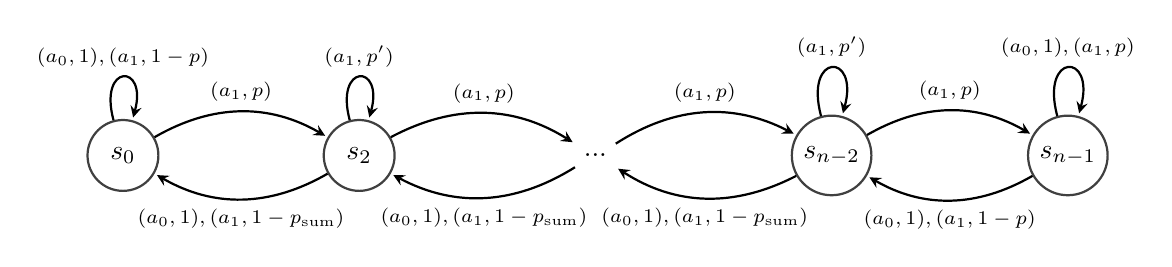
\begin{tikzpicture}[->,>=stealth,shorten >=1pt,auto,node distance=2cm,thick]
    \tikzstyle{state}=[circle,thick,draw=black!75,minimum size=9mm,inner sep=1mm]
    
    \node[state] (A) at (0,0) {$s_0$};
    \node[state] (B) at (3,0) {$s_2$};
    \node (C) at (6,0) {...};
    \node[state] (D) at (9,0) {$s_{n-2}$};
    \node[state] (E) at (12,0) {$s_{n-1}$};
    
    \path (A) edge [loop above] node[midway,above, font=\scriptsize] {$(a_0,1),(a_1,1-p)$} (A)
              edge [bend left] node[midway,above, font=\scriptsize] {$(a_1,p)$} (B)
          (B) edge [bend left] node[midway,below, font=\scriptsize] {$(a_0,1), (a_1,1-p_{\rm sum})$}  (A)
              edge [loop above] node[midway,above, font=\scriptsize] {$(a_1,p')$} (B)
              edge [bend left] node[midway,above, font=\scriptsize] {$(a_1,p)$}  (C)
          (C) edge [bend left] node[midway,below, font=\scriptsize] {$(a_0,1), (a_1,1-p_{\rm sum})$}  (B)
              edge [bend left] node[midway,above, font=\scriptsize]{$(a_1,p)$} (D)
          (D) edge [bend left] node[midway,below, font=\scriptsize] {$(a_0,1), (a_1,1-p_{\rm sum})$} (C)
              edge [loop above] node[midway,above, font=\scriptsize] {$(a_1,p')$}(D)
              edge [bend left] node[midway,above, font=\scriptsize]{$(a_1,p)$} (E)
          (E) edge [bend left] node[midway,below, font=\scriptsize] {$(a_0,1), (a_1,1-p)$}  (D)
              edge [loop above] node[midway,above, font=\scriptsize] {$(a_0,1),(a_1,p)$} (E);
    
    \end{tikzpicture}
    \caption{{\tt Riverswim} environment \cite{strehl2004empirical}. Each tuple $(a,p)$ represents the action $a$ that triggers the transition and the probability $p$ of that event.}
    \label{fig:riverswim_env}
\end{figure}
   % \draw[->] (s0) edge[bend left]  node[midway,above, font=\scriptsize] {$(a_1,0.3,\theta)$} (s1) ;


\paragraph{Forked Riverswim.} The Forked RiverSwim environment \cite{russo2023model} is a variation of the traditional RiverSwim reinforcement learning benchmark, designed to test more complex exploration strategies. In this variant, the state space branches into multiple paths, resembling a river that forks. At intermediate states the agent can switch between the forks, while the end states are not connected.  This variant requires the agent to make more sophisticated decisions to explore the environment. This setup increases the sample complexity and challenges the agent's ability to generalize across different paths within the environment.

In \cref{fig:forkedriverswim_env} is shown a depiction of the environment. There are a total of $2n+1$ states, and two parameters $p,p'\in (0,1)$,  so that $p_{\rm sum}=p+p'<1$. In the figure, each tuple $(a,p)$ represents the  action $a$ that triggers the transition and the probability $p$ of that event. The agent starts in state $s_0$, and in every state can chose between three actions $\{a_0,a_1, a_2\}$. For small values of $p$ it becomes difficult for the agent to swim right  in both forks, and larger values of $p'$ can also hinder the progress. As in Riverswim, swimming towards the left is easier, since the probability of $P(s_{i-1}|s_i, a_0)=1$. For the experiments, we used $n\in\{8,10,15\}, p=0.7, p'=6(1-p)/7$.


\begin{figure}[h]
    \centering
    \resizebox{.75\linewidth}{!}{%
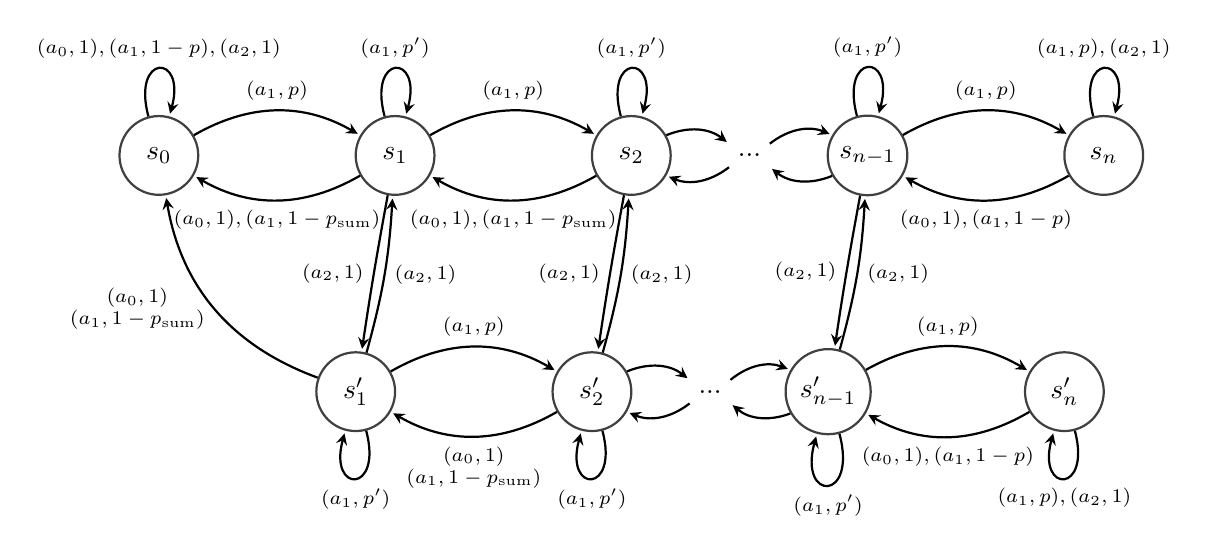
\begin{tikzpicture}[->,>=stealth,shorten >=1pt,auto,node distance=3cm,thick]
\tikzstyle{state}=[circle,thick,draw=black!75,minimum size=10mm,inner sep=1mm]

\node[state] (A) at (0,0) {$s_0$};
\node[state] (B) at (3,0) {$s_1$};
\node[state] (C) at (6,0) {$s_2$};
\node[state] (D) at (9,0) {$s_{n-1}$};
\node[state] (E) at (12,0) {$s_{n}$};
\node[state] (F) at (2.5,-3) {$s_1'$};
\node[state] (G) at (5.5,-3) {$s_2'$};
\node[state] (H) at (8.5,-3) {$s_{n-1}'$};
\node[state] (I) at (11.5,-3) {$s_{n}'$};
\node (C1) at (7.5,0) {...};
\node (C2) at (7,-3) {...};

\path (A) edge [loop above] node[midway,above, font=\scriptsize] {$(a_0,1),(a_1,1-p),(a_2,1)$} (A)
          edge [bend left] node[midway,above, font=\scriptsize] {$(a_1,p)$} (B)
          %edge [bend right=10] node[midway,below, font=\scriptsize] {0.1} (F)
      (B) edge [loop above] node[midway,above, font=\scriptsize] {$(a_1,p')$} (B)
          edge [bend left] node[midway,above, font=\scriptsize] {$(a_1,p)$} (C)
          edge [bend right=1] node[midway,left, font=\scriptsize] {$(a_2,1)$} (F)
          edge [bend left] node[midway,below, font=\scriptsize] {$(a_0,1),(a_1,1-p_{\rm sum})$}   (A)
      (C) edge [loop above] node[midway,above, font=\scriptsize] {$(a_1,p')$} (C)
          edge [bend left]  (C1)
          edge [bend right=1] node[midway,left, font=\scriptsize] {$(a_2,1)$}  (G)
          edge [bend left] node[midway,below, font=\scriptsize] {$(a_0,1),(a_1,1-p_{\rm sum})$} (B)
      (C1) edge [bend left]  (D)
           edge [bend left]  (C)
      (D) edge [loop above] node[midway,above, font=\scriptsize] {$(a_1,p')$} (D)
          edge [bend left] node[midway,above, font=\scriptsize] {$(a_1,p)$} (E)
          edge [bend left]  (C1)
          edge [bend right=1] node[midway,left, font=\scriptsize] {$(a_2,1)$} (H)
      (E) edge [loop above] node[midway,above, font=\scriptsize] {$(a_1,p),(a_2,1)$} (E)
           edge [bend left] node[midway,below, font=\scriptsize] {$(a_0,1),(a_1,1-p)$} (D)
           
      (F) edge [loop below] node[midway,below, font=\scriptsize] {$(a_1, p')$} (F)
          edge [bend left] node[midway,above, font=\scriptsize] {$(a_1,p)$} (G)
          edge [bend left=30] node[midway,left, align=center,font=\scriptsize] {$(a_0,1)$\\$(a_1,1-p_{\rm sum})$} (A)
          edge [bend right=6] node[midway,right, font=\scriptsize] {$(a_2,1)$} (B)
      (G) edge [loop below] node[midway,below, font=\scriptsize]  {$(a_1, p')$} (G)
          edge [bend left]  (C2)
          edge [bend left] node[midway,below, align=center, font=\scriptsize] {$(a_0,1)$\\$(a_1,1-p_{\rm sum})$} (F)
          edge [bend right=6] node[midway,right, font=\scriptsize] {$(a_2,1)$}  (C)
      (C2) edge [bend left]  (H)
           edge [bend left]  (G)
          
      (H) edge [loop below] node[midway,below, font=\scriptsize] {$(a_1,p')$} (H)
          edge [bend right=6] node[midway,right, font=\scriptsize] {$(a_2,1)$} (D)
          edge [bend left]  (C2)
          edge [bend left] node[midway,above, font=\scriptsize] {$(a_1,p)$} (I)
      (I) edge [loop below] node[midway,below, font=\scriptsize] {$(a_1,p),(a_2,1)$} (I)
          edge [bend left] node[midway,below, font=\scriptsize] {$(a_0,1),(a_1,1-p)$}  (H);

\end{tikzpicture}}
    \caption{{\tt Forked Riverswim} environment \cite{russo2023model}. Each tuple $(a,p)$ represents the action $a$ that triggers the transition and the probability $p$ of that event.}
    \label{fig:forkedriverswim_env}
\end{figure}


\paragraph{Double Chain.} The Double Chain environment \cite{Kaufmann21a} consists of two chains, similarly to the Forked Riverswim. The main difference consists in the fact that it is not possible to switch between the two chains, and intermediate states are transient (there is no parameter $p'$).


In \cref{fig:doublechain_env} is shown a depiction of the environment. There are a total of $2n+1$ states, and one parameters $p\in (0,1)$. In the figure, each tuple $(a,p)$ represents the  action $a$ that triggers the transition and the probability $p$ of that event. The agent starts in state $s_0$, and in every state can chose between two actions $\{a_0,a_1\}$. For small values of $p$ it becomes difficult for the agent to move to the end of the chain  in both chains. For the experiments, we used $n\in \{8,10,15\}, p=0.7$.



\begin{figure}[h]
    \centering
    \resizebox{.75\linewidth}{!}{%
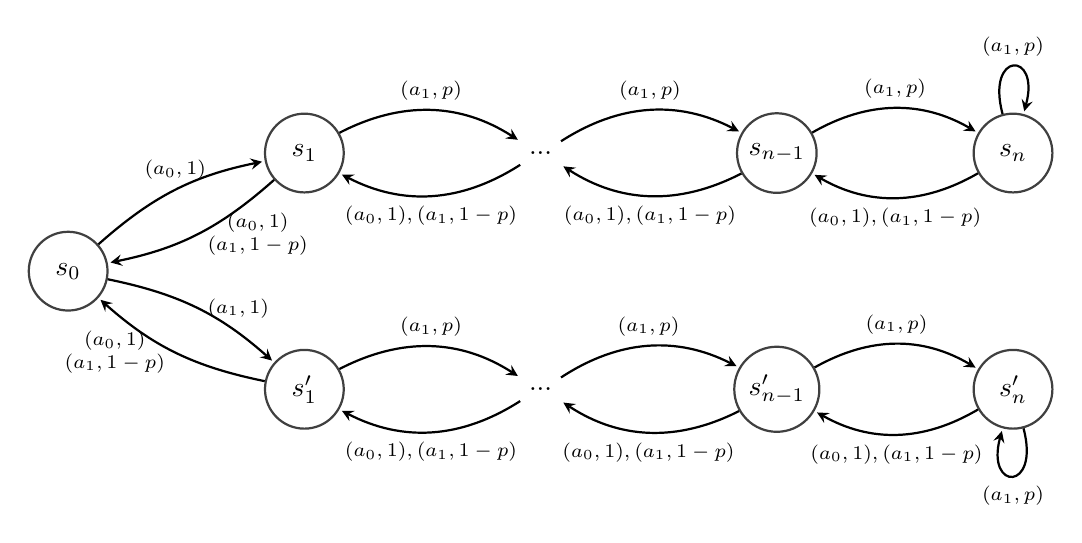
\begin{tikzpicture}[->,>=stealth,shorten >=1pt,auto,node distance=3cm,thick]
\tikzstyle{state}=[circle,thick,draw=black!75,minimum size=10mm,inner sep=1mm]

\node[state] (A) at (0,-1.5) {$s_0$};
\node[state] (B) at (3,0) {$s_1$};
\node[state] (D) at (9,0) {$s_{n-1}$};
\node[state] (E) at (12,0) {$s_{n}$};
\node[state] (F) at (3,-3) {$s_1'$};
\node[state] (H) at (9,-3) {$s_{n-1}'$};
\node[state] (I) at (12,-3) {$s_{n}'$};
\node (C1) at (6,0) {...};
\node (C2) at (6,-3) {...};

\path (A) edge [bend left=15] node[midway,above, font=\scriptsize] {$(a_0,1)$} (B)
          edge [bend left=15] node[midway,right, font=\scriptsize] {$(a_1,1)$} (F)
      (B) edge [bend left] node[midway,above, font=\scriptsize] {$(a_1,p)$} (C1)
          edge [bend left=15] node[midway,right, align=center,font=\scriptsize] {$(a_0,1)$\\$(a_1,1-p)$}   (A)

      (C1) edge [bend left]  node[midway,above, font=\scriptsize] {$(a_1,p)$}(D)
           edge [bend left] node[midway,below, font=\scriptsize] {$(a_0,1),(a_1,1-p)$}  (B)
      (D) edge [bend left] node[midway,above, font=\scriptsize] {$(a_1,p)$} (E)
          edge [bend left] node[midway,below, font=\scriptsize] {$(a_0,1),(a_1,1-p)$} (C1)
      (E) edge [loop above] node[midway,above, font=\scriptsize] {$(a_1, p)$} (E)
           edge [bend left] node[midway,below, font=\scriptsize] {$(a_0,1),(a_1,1-p)$} (D)
           
      (F) edge [bend left] node[midway,above, font=\scriptsize] {$(a_1,p)$} (C2)
          edge [bend left=15] node[midway,left, align=center,font=\scriptsize] {$(a_0,1)$\\$(a_1,1-p)$} (A)

      (C2) edge [bend left] node[midway,above, font=\scriptsize] {$(a_1,p)$} (H)
           edge [bend left] node[midway,below, font=\scriptsize] {$(a_0,1),(a_1,1-p)$} (F)
          
      (H) edge [bend left] node[midway,below, font=\scriptsize] {$(a_0,1),(a_1,1-p)$}  (C2)
          edge [bend left] node[midway,above, font=\scriptsize] {$(a_1,p)$} (I)
      (I) edge [loop below] node[midway,below, font=\scriptsize] {$(a_1,p)$} (I)
          edge [bend left] node[midway,below, font=\scriptsize] {$(a_0,1),(a_1,1-p)$}  (H);

\end{tikzpicture}
}
    \caption{{\tt Double Chain} environment \cite{Kaufmann21a} . Each tuple $(a,p)$ represents the action $a$ that triggers the transition and the probability $p$ of that event.  }
    \label{fig:doublechain_env}
\end{figure}




\paragraph{NArms.} This environment is an adaptation to $N$ arms of the original {\tt 6Arms} environment from  \cite{strehl2004empirical}. Differently from the previous environments, this is a bandit-like environment, where the agent is presented with $n$ different actions (or arms) to choose from. The agent starts in a state $s_0$ and selects an arm $a_i$. Upon selecting an arm, the agent may transition to corresponding state $s_i$. Certain arms are more difficult to observe, in the sense that the transition probability is lower. This property mimics the  probability of collecting a reward in a bandit problem.
In \cref{fig:narms_env} is shown a depiction of the environment. There are a total of $n+1$ states, and one parameters $p_0\in (0,1)$. In the figure, each tuple $(a,p)$ represents the  action $a$ that triggers the transition and the probability $p$ of that event. The notation  $a_{n_0:n_0+n}$ indicates  all the actions in $\{a_{n_0},\dots,a_{n_0+n}\}$.
The agent starts in state $s_0$, and in every state she can select between $n$ actions $\{a_0,a_1,\dots, a_{n-1}\}$. For small values of $p_0$ it becomes difficult for the agent to move to different states. Similarly, it is harder to navigate to states $s_i$ for large values of $n$. We used $p_0=0.7$ and $n\in \{10,20,30\}$.





\begin{figure}[h]
    \centering
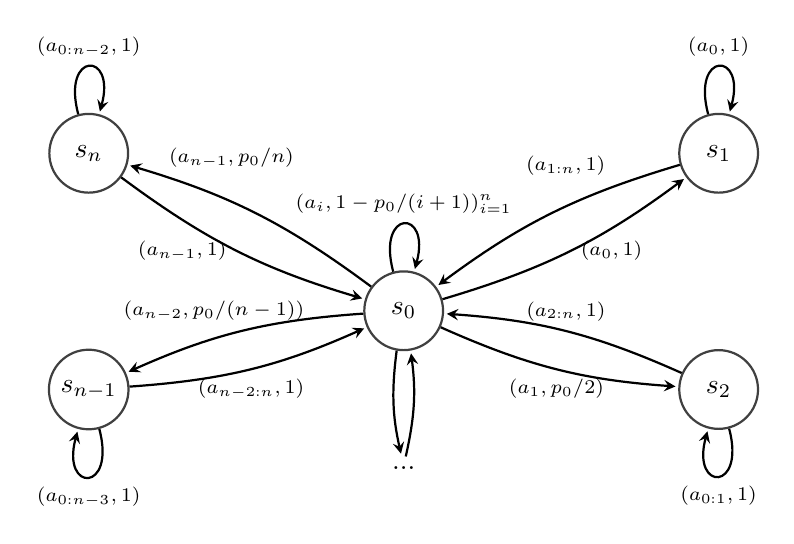
\begin{tikzpicture}[->,>=stealth,shorten >=1pt,auto,node distance=3cm,thick]
\tikzstyle{state}=[circle,thick,draw=black!75,minimum size=10mm,inner sep=1mm]

% Central hub
\node[state] (A) at (0,0) {$s_0$};

% Arms
\node[state] (B1) at (4,2) {$s_1$};
\node[state] (B2) at (4,-1) {$s_2$};
\node  (C) at (0,-2) {...};
\node[state] (B5) at (-4,2) {$s_n$};
\node[state] (B6) at (-4,-1) {$s_{n-1}$};

\path (A) edge [bend right=10] node[midway,right, font=\scriptsize] {$(a_0,1)$} (B1)
          edge [bend right=10] node[midway,below, font=\scriptsize] {$(a_1,p_0/2)$} (B2)
          edge [bend right=10] (C)
          edge [bend right=10] node[midway,right, font=\scriptsize,yshift=20pt,xshift=-35pt] {$(a_{n-1}, p_0/n)$} (B5)
          edge [bend right=10] node[midway,above, font=\scriptsize, xshift=-10pt] {$(a_{n-2}, p_0/(n-1))$} (B6)
          edge [loop above] node[midway,above, font=\scriptsize] {$(a_i, 1- p_0/(i+1))_{i=1}^n$} (A)
      (B1) edge [bend right=10] node[midway,above, font=\scriptsize,yshift=10pt,xshift=5pt] {$(a_{1:n},1)$} (A)
           edge [loop above] node[midway,above, font=\scriptsize] {$(a_{0},1)$} (B1)
      (B2) edge [bend right=10] node[midway,above, font=\scriptsize] {$(a_{2:n},1)$} (A)
           edge [loop below] node[midway,below, font=\scriptsize] {$(a_{0:1},1)$} (B2)

      (C) edge [bend right=10] node[midway,below, font=\scriptsize] {} (A)

      (B5) edge [bend right=10] node[midway,left, font=\scriptsize] {$(a_{n-1},1)$} (A)
       edge [loop above] node[midway,above, font=\scriptsize] {$(a_{0:n-2},1)$} (B5)
      (B6)  edge [bend right=10] node[midway,below, font=\scriptsize] {$(a_{n-2:n},1)$} (A)
      edge [loop below] node[midway,below, font=\scriptsize] {$(a_{0:n-3},1)$} (B6);

\end{tikzpicture}

    \caption{{\tt NArms} environment. Each tuple $(a,p)$ represents the action $a$ that triggers the transition and the probability $p$ of that event. In the figure the notation $a_{n_0:n_0+n}$ indicates  all the actions in $\{a_{n_0},\dots,a_{n_0+n}\}$. In state $s_0$ the probability to remain in $s_0$ for any action $a_i$ is $P(s_0|s_0,a_i)=1-p_0/(i+1)$, with the exception that $P(s_0|s_0,a_0)=0$.}
    \label{fig:narms_env}
\end{figure}



\subsection{Algorithm Details}\label{app:algorithms}
In this section we briefly explain the mechanisms of each algorithm used in the experiments, and, in case, their adaptation. Note that for all algorithms we evaluated the policies by  using the MDP estimate $M_t$ through policy evaluation.


\paragraph{ Noisy Policy (Uniform).} This method simply computes a mixture of the target policies $\pi_{\rm mix}(a|s) = \frac{|\{\pi\in \Pi: \pi(s)=a\}|}{|\Pi|}$, which is then mixed with a uniform policy $\pi_u$ with a constant mixing factor $\varepsilon_t=0.3$. The resulting behavior policy is $\pi_b =(1-\varepsilon_t)\pi_{\rm mix} +\varepsilon_t \pi_u$.

\paragraph{Noisy Policy (Visitation).} This method is similar to the previous one, but the mixing factor is not constant anymore. We take a mixing factor that is $\epsilon_t=1/N_t(s_t)$, which based on the number of visits to state $s_t$. The resulting behavior policy is $\pi_b =(1-\varepsilon_t)\pi_{\rm mix} +\varepsilon_t \pi_u$.

\paragraph{SF-NR \cite{mcleod2021continual}.} This is an algorithm for multi-task policy evaluation based on the Successor Representation. The pseudo-steps of the algorithm can be found in \cref{algo:sfnr}. The method maintains a successor representation $\psi_{\pi,t}$ for each policy $\pi$, as well as a behavior policy $\pi_\beta$. These are learned using TD-learning, and the behavior policy uses the variation between $\psi_{\beta,t+1}$ and $\psi_{\beta,t}$ as a reward. 
In our experiment we used a temperature $T=2$ and a discount factor for the successor representation $\gamma_\psi=0.99$.

\begin{algorithm}[h]
	\caption{{\tt SF-NR}}
	\label{algo:sfnr}
    \small
	\begin{algorithmic}[1]
    \REQUIRE Discount factor $\gamma$; Temperature $T$; Successor discount factor $\gamma_\psi$; policy set $\Pi$.
    \STATE Set $\pi_\beta(\cdot|s)={\cal U}(\{1,\dots,A\})$ for all states $s$.
    \STATE Set $\psi_{\pi,1}(s,a)=1$ for all $(s,a)$.
    \WHILE{not done} 
            \STATE Compute $\hat \pi_\beta(\cdot|s_t) = {\tt Softmax}(\pi_\beta(\cdot|s_t)/T)$
            \STATE Sample $a_t$ from $(1-\varepsilon_t)\hat \pi_\beta(\cdot|s_t)  +\varepsilon_t/A$ and observe $s_{t+1}\sim P(\cdot|s_t,a_t)$.
            \FOR{$\pi \in \Pi$}
                \STATE Compute $\delta_t=1+\gamma_\psi \psi_{\pi,t}(s_{t+1},\pi(s_{t+1}))-\psi_{\pi,t}(s_t,a_t)$
                \STATE Set $\psi_{\pi,t+1}(s_t,a_t)= \psi_{\pi,t}(s_t,a_t) + \alpha_t \delta_t$, where $\alpha_t=1/N_t(s_t,a_t)$.
            \ENDFOR
            \STATE Compute $\delta_{\psi,t}=1/|\Pi| \sum_{\pi\in \Pi}\|{\rm Vec}(\psi_{\pi,t+1})- {\rm Vec}(\psi_{\pi,t})\|_1$.
            \STATE Update $\pi_\beta(a_t|s_t)\gets \pi_\beta(a_t|s_t)+ \alpha_t\left(\delta_{\psi,t}+ \gamma \max_a\pi_\beta(a|s_{t+1}) - \pi_\beta(a_t|s_t)\right)$, where $\alpha_t=1/N_t(s_t,a_t)$.
            \STATE Update MDP estimate $M_t$ and set $t\gets t+1$.
            \ENDWHILE{}
	\end{algorithmic}
\end{algorithm}



\paragraph{GVFExplorer \cite{jain2024adaptive}.}  This method considers variance-based exploration strategy for learning general value functions \cite{sutton2011horde} based on minimizing the MSE. 
 The pseudo-steps of the algorithm can be found in \cref{algo:gvf}. 
Given the current estimate of the MDP $M_t$, the method estimates ${\rm Var}_{s,a}^\pi(t)$, the variance of the return $G^\pi=r_1+\gamma r_2+\gamma^2 r_3+\dots$ under $\pi$ staring from $(s,a)$, $\forall\pi\in \Pi, (s,a)\in \statespace\times\actionspace$. Then, a behavior policy is computed as $
\pi_\beta(a|s) = \frac{\sqrt{\sum_{\pi\in\Pi} \pi(a|s)  {\rm Var}_{s,a}^\pi(t)}}{\sum_b\sqrt{\sum_{\pi\in\Pi} \pi(b|s)  {\rm Var}_{s,b}^\pi(t)}}$. Lastly, we mix this policy with a uniform policy. For this method we used a fixed mixing factor $\varepsilon=0.3$ (we did not use a visitation based mixing factor because performance deteriorated).





\begin{algorithm}[h]
	\caption{{\tt GVFExplorer}}
	\label{algo:gvf}
    \small
	\begin{algorithmic}[1]
    \REQUIRE Mixing factor $\varepsilon$, policy set $\Pi$.
    \STATE Set ${\rm Var}_{s,a}^\pi(1)=1$ for all $(s,a)\in \statespace\times\actionspace, \pi\in \Pi$.
    \WHILE{not done} 
            \STATE Set $\pi_\beta(a|s) = \frac{\sqrt{\sum_{\pi\in\Pi} \pi(a|s)  {\rm Var}_{s,a}^\pi(t)}}{\sum_b\sqrt{\sum_{\pi\in\Pi} \pi(b|s)  \rm Var_{s,b}^\pi(t)}}$
            \STATE Sample $a_t$ from $(1-\varepsilon) \pi_\beta(\cdot|s_t)  +\varepsilon/A$ and observe $s_{t+1}\sim P(\cdot|s_t,a_t)$.
            \STATE Update MDP estimate $M_t$, variance estimates $\{{\rm Var}^\pi(t)\}_{\pi\in \Pi}$ and set $t\gets t+1$.
            \ENDWHILE{}
	\end{algorithmic}
\end{algorithm}
Note that $\pi_\beta$ is similar to the generative solution in \cref{eq:T_epsilon_omega} (i.e., $\Omega(M)=\Delta(\statespace\times\actionspace)$). In fact, {\tt GVFExplorer}  neglects the forward equations when deriving $\pi_\beta$. The resulting solution does not take into account the dynamics induced by the behavior policy, effectively making it a generative method (compare with the generative solution proved in \cite{al2021adaptive,russo2023model}). We believe this is due to a term being omitted  in the proof of \citet[Theorem 4.1]{jain2024adaptive}  that accounts for how changes in the state distribution induced by the behavior policy impact the variance. 
  

\paragraph{MR-NaS.} For \mrnas{} we computed the exploration strategy $\omega_t^\star$ every $500$ steps in the environment, to avoid excessive computational burden.
The policy is then mixed with a forcing policy that is $\pi_{f,t}(\cdot|s)=\texttt{softmax}\left(-\beta_t(s) N_t(s,\cdot)\right)$
with $\beta_t(s) = \frac{\beta  \log(N_t(s))}{\max_a |N_t(s,a) - \min_b N_t(s,b)|}, \beta\in [0,1]$ and  $({\tt softmax}(x))_i=e^{x_i}/\sum_j e^{x_j}$ for a vector $x$. This choice encourages to select under-sampled actions for $\beta > 0$, while for $\beta=0$ we obtain a uniform forcing policy $\pi_{f,t}(a|s)=1/A$. 
 We then mix $\omega_t^\star$ with $\pi_{f,t}$ using a mixing factor $\epsilon_t = 1/\max(1,N_t(s_t))^\alpha$, with $N_t(s) = \sum_a N_t(s,a)$. The values $\alpha,\beta$ need to guarantee $\alpha+\beta\leq 1$ \cite{russomulti}, hence we chose $\alpha=0.99$ and $\beta=0.01$.

\subsection{Additional Results}\label{app:additional_results}
In this sub-section we report additional  results. To run reproduce the results, we refer the reader to the {\tt README.md} file in the supplementary material. In \cref{fig:app:multi_pol_multi_rew} are reported the results for the multi-reward multi-policy case with various sizes of the state space. Similarly, in \cref{fig:app:rew_free_multi_pol} are reported the reward-free results for the multi-policy case, and in \cref{fig:app:single_pol_rewfree} the results for the single-policy reward-free case. Experiments were run over $10^6$ time-steps, with $30$ seeds. Confidence intervals were computed using bootstrap \cite{efron1992bootstrap}.

\begin{figure}
    \centering
    \includegraphics[width=\linewidth]{figures/1000000_multi_policy_multi_reward_abs_error_small.pdf}
    \includegraphics[width=\linewidth]{figures/1000000_multi_policy_multi_reward_abs_error_medium.pdf}
    \includegraphics[width=\linewidth]{figures/1000000_multi_policy_multi_reward_abs_error_large.pdf}
    \caption{Multi-reward multi-policy evaluation for different sizes of the MDPs: from top to bottom the state space size is $15, 20, 30$. Shaded curves represent 95\% confidence intervals.}
    \label{fig:app:multi_pol_multi_rew}
\end{figure}

\begin{figure}
    \centering
    \includegraphics[width=\linewidth]{figures/1000000_multi_policy_rewfree_abs_error_small.pdf}
    \includegraphics[width=\linewidth]{figures/1000000_multi_policy_rewfree_abs_error_medium.pdf}
    \includegraphics[width=\linewidth]{figures/1000000_multi_policy_rewfree_abs_error_large.pdf}
    \caption{Reward-Free multi-policy evaluation for different sizes of the MDPs: from top to bottom the state space size is $15, 20, 30$. Here we depict the average error over the canonical basis  ${\cal R}_{\rm canonical}$. Shaded curves represent 95\% confidence intervals.}
    \label{fig:app:rew_free_multi_pol}
\end{figure}

\begin{figure}
    \centering
    \includegraphics[width=\linewidth]{figures/1000000_single_policy_rewfree_abs_error_small.pdf}
    \includegraphics[width=\linewidth]{figures/1000000_single_policy_rewfree_abs_error_smedium.pdf}
    \includegraphics[width=\linewidth]{figures/1000000_single_policy_rewfree_abs_error_large.pdf}
    \caption{Reward-Free single-policy evaluation for different sizes of the MDPs: from top to bottom the state space size is $15, 20, 30$. Here we depict the average error over the canonical basis  ${\cal R}_{\rm canonical}$. Shaded curves represent 95\% confidence intervals.}
    \label{fig:app:single_pol_rewfree}
\end{figure}
We have introduced iVISPAR, a novel interactive multi-modal benchmark designed to evaluate the spatial reasoning capabilities in 3D vision of VLMs acting as agents. The benchmark, centered on the Sliding Geom Puzzle, evaluates VLMs' abilities in logical planning, spatial awareness, and multi-step problem-solving, aiming to reflect real-world spatial reasoning. Our evaluation tested a suite of state-of-the-art open-source and closed-source VLMs on a dataset of board configurations, scaled across two levels of complexity. We compared them to baselines for human capabilities, optimal and random agents, providing insight into their performance under varying conditions.

\subsubsection*{Acknowledgement} The authors acknowledge support by the state of Baden-Würt\-tem\-berg through bwHPC, and the Hellenic Foundation for Research and Innovation (H.F.R.I.) under the \enquote{2nd Call for H.F.R.I.~Research Projects to support Post-Doctoral Researchers} (project number: $01247$). 

\bibliographystyle{ieeetr}
\bibliography{dual_norm_literature.bib}

\end{document}